\chapter{Filter Graph Editor}
\label{grapheditor}

The filter graph editor allows complex signal processing pipelines to be developed in a graphical fashion.

It may be accessed from the \menustyle{Window / Filter Graph} menu item.

The leftmost column shows all of the input channels which may be used as data sources for the filter graph. Filter
nodes are automatically placed in columns such that data flows from left to right, with inputs at the left and outputs
at the right of each node.

Nodes may be dragged vertically within their column by using the left mouse button, however the horizontal position of
each node is fixed.

To make a connection, click on the source node's output and then on the destination node's input. To cancel an
in-progress connection, simply click anywhere outside a node.

\begin{figure}[H]
\centering
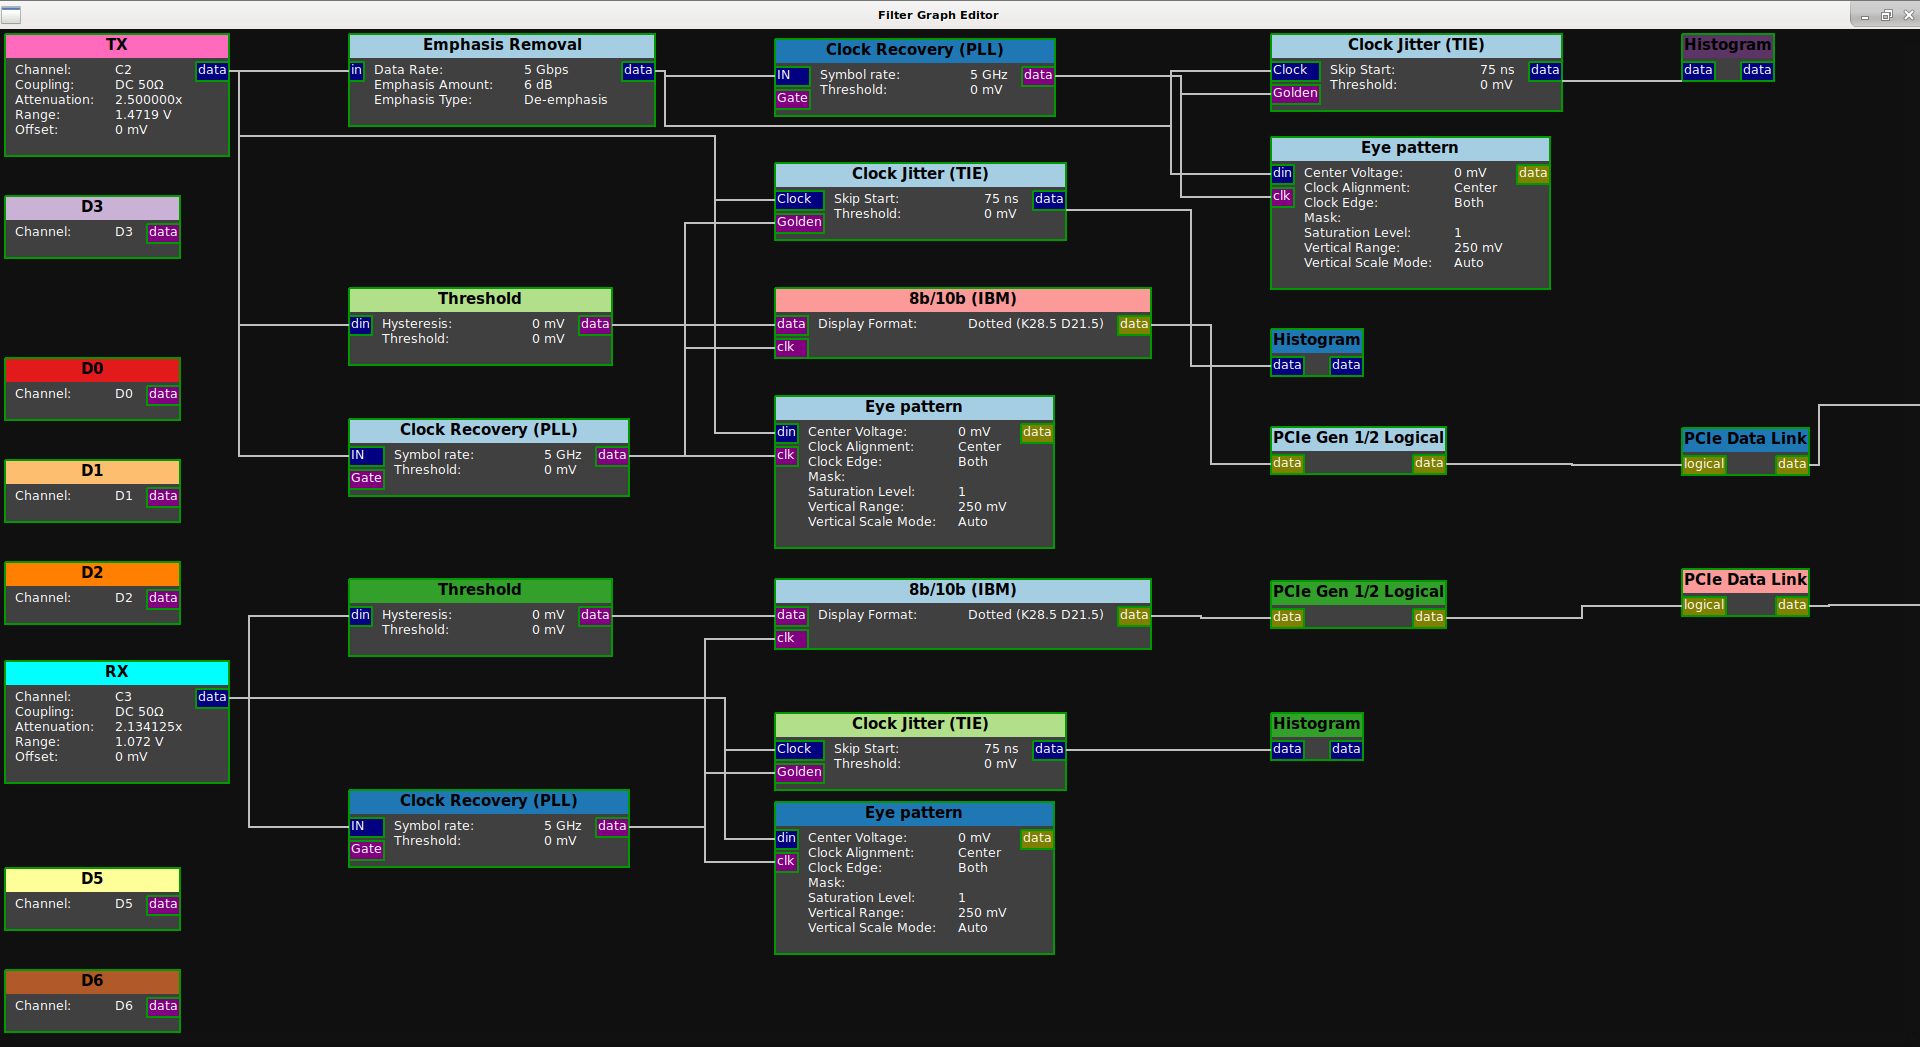
\includegraphics[width=17cm]{images/graph-editor.png}
\caption{Filter graph editor view}
\label{graph-editor}
\end{figure}

The title bar of each node in the graph is color coded to match the channel's color in the waveform view.

Input and output ports are color coded according to the type of data. The colors are configurable under the
\menustyle{Appearance / Filter Graph} preference category; the default assignment is dark blue for analog, purple for
digital, and olive for protocol decodes and other non-primitive types.
